\iffalse \bibliography{include/backmatter/references} \fi
\chapter{Methodology}

This report seeks to gather relevant literature regarding the topic of leadership within agile software development projects by implementing a snowballing search approach. The snowballing search approach is complementary to the traditional database search. It aims to allow for a systematic approach to finding related work by studying the reference list and citations of a start set of related literature to identify further relevant literature. The snowballing search approach is implemented to ensure good coverage of current literature in a systematic way.\\

The paper by \cite{Wohlin:2014:GSS:2601248.2601268} presents the guidelines for the procedures used in this report for investigating and gathering relevant literature. Figure \ref{snow} depicts the procedures included in the snowballing search approach which involve (i) choosing a number of papers referred to as the start set, (ii) apply forward snowballing on each paper chosen for the start set, and (iii) apply backward snowballing on each paper chosen for the start set. This process is repeated until no new papers are found in the identified pool of relevant literature.\\

\begin{figure}[ht]
\centering
     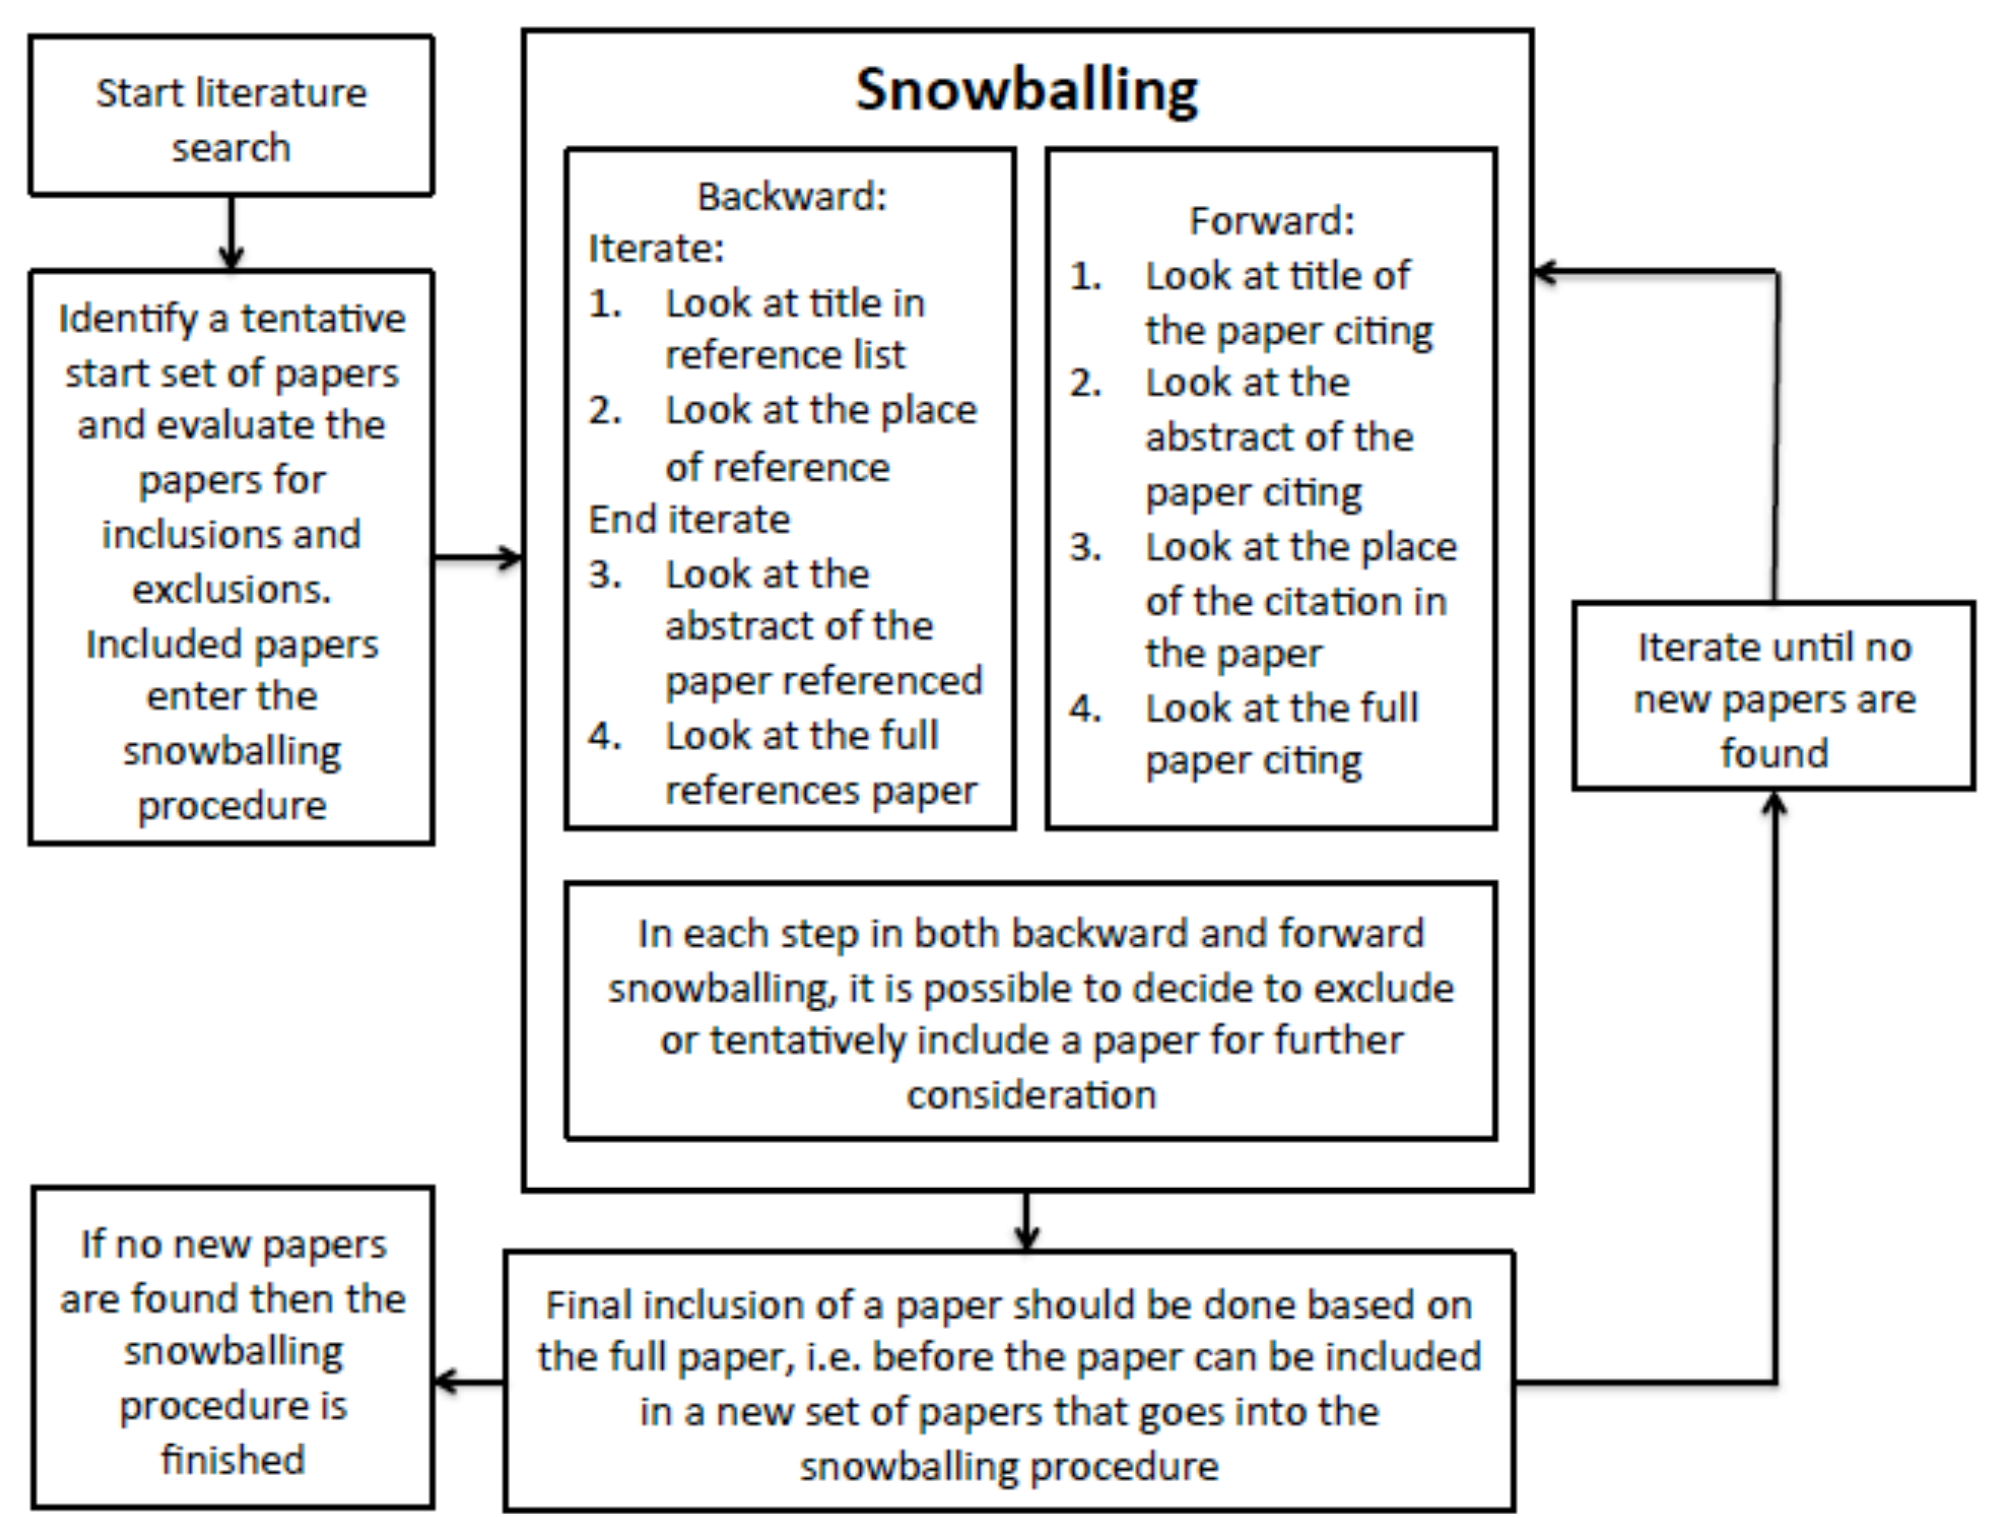
\includegraphics[width=0.8\textwidth]{./fig/snowballing.png}
      \caption{Snowballing guidelines \cite{Wohlin}.}
       \label{snow}
\end{figure}

To initiate the snowball search a set of keywords are selected from the research questions which are aimed specific and detailed in regards to this study. Selecting precise keywords are crucial to ensure that the start set is highly relevant to this research as a broad set of keywords may generate papers which are outside the scope of this study. After a search string is identified it is applied to a database which covers multiple publishers to ensure the start set is complete without any publisher biased. To further ensure that the start set is specific to topic of the study, each paper is screened and included based on inclusion and exclusion criteria.\\

Next, backward- and forward snowballing is applied on the start set to gather relevant literature within the chosen field. Backward snowballing is the process of studying the reference list of a paper from the start set to identify further relevant papers. Looking at the place of reference and reading the title and abstract of the paper cited is firstly done to recognise whether or not the cited paper is relevant for this study. Inclusion and exclusion criteria are applied to the paper. The entire paper is studied if the paper is relevant and included in this study. Forward snowballing is the process of studying papers which cite the paper under inspection. The process of reading and studying the relevance of the citing paper is done. The entire paper is further studied if included for this study.\\


\begin{table}[ht]
\centering
\caption{Start set}
\label{tab:start-set}
\renewcommand{\arraystretch}{1.2}
\begin{tabu}{l|l}
\textbf{Paper No.} & \textbf{Citation}\\ \tabucline[2pt]{-}

\end{tabu}
\end{table}